\textnormal{
Transform the project requirements into a system flow diagram, specifyng the different algorithms, data types and structures required for processing and their associated operations.  
The deliverables for this stage include the system flow diagram containing a graphical representation and  textual descriptions of the corresponding data trasnformations, high level pseudo code of the overall system operation, and overall system time and space complexity.}

%\begin{itemize} 
%\item{ }
%A brief textual description of the overall flow diagram (along with its functional operation in the different user scenarios described in the first stage of the project).
%\item{ }
%A specification of each algorithm and associated data structures together with its entities, attributes, and operations ( include an English description of how they relate to your user scenario(s)).

%\end{itemize}
Please insert your deliverables for Stage2 as follows:
\begin{itemize} 
\item{  Short Textual Project Description. }
Please insert here the flow diagram textual description here together with its overall time and space complexity.
\item{ Flow Diagram. }
\begin{figure}[h]
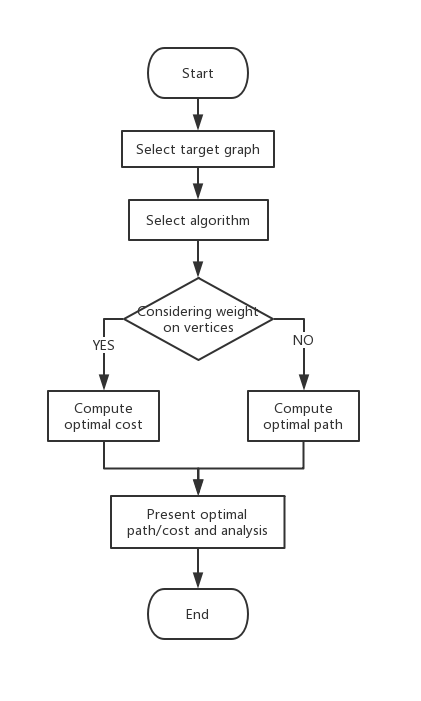
\includegraphics[width=\linewidth]{Systemflowchart.png}
\caption{System Flow Diagram}
\label{fig1}
\end{figure}
\begin{figure}[h]
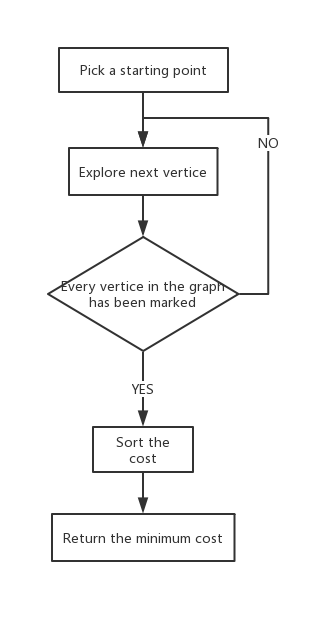
\includegraphics[width=\linewidth]{Method1.jpg}
\caption{Algorithm 1: Exhaustion}
\label{fig2}
\end{figure}
\begin{figure}[h]
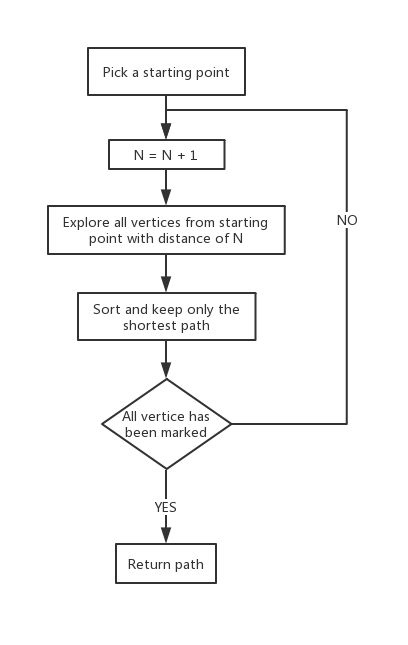
\includegraphics[width=\linewidth]{Method2.png}
\caption{Algorithm 2: Dynamic Programming}
\label{fig3}
\end{figure}
\begin{figure}[h]
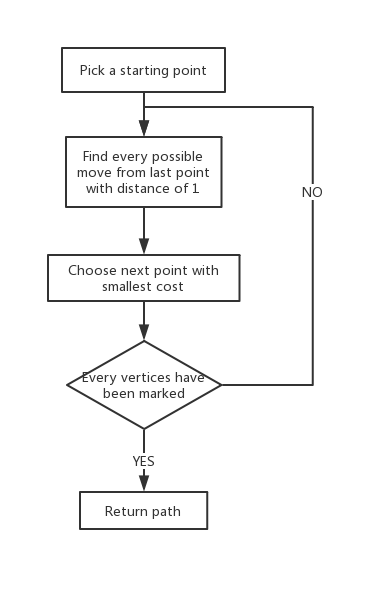
\includegraphics[width=\linewidth]{Method3.png}
\caption{Algorithm 3: Greedy Algorithm}
\label{fig4}
\end{figure}
Please insert your system Flow Diagram here.
\item{ High Level Pseudo Code System Description. }
\\
Initially, a complete directed graph is given. It has weight on edges and vertices.(distance cost and mass cost)
\\
\par
\setlength{\parskip}{0.5\baselineskip}
1. For small n, we can use the easiest method which is exhaustion:
\begin{quote}
\#Set the starting point
\\
\#Generate all permutations of visiting n vertices
\\
\#Keep track of the minimum cost considering weight of both edges and vertices
\\
\#Return the minimum cost and its path
\end{quote}
This method has time and space complexity of O(n!) since there are n! permutations in total(That's why it only works for small n). This method will be used to verify our result using the other two methods.
\par
2. A more realistic and effective way is dynamic programming:
\begin{quote}
\#Set the starting point
\\
\#Start with visiting v=2 vertices in total.(1 starting point and 1 other point)
\\
\#Calculate the cost of each path and store the result.(All vertices visited already, the last vertex visited, total distance cost, total mass cost, mass carried)
\\
\#If more than one path share the same visited vertices and last vertex, only keep the one with minimum cost
\\
\#Continue with v=3 using the result of v=2
\\
\#Repeat the previous steps for v=4, 5, 6... until v=n
\\
\#The last step is adding the edge from the end point back to the starting point and find the minimum cost
\\
\#Return the minimum cost and its path
\end{quote}
This method is much faster than the first one and it should give the correct final answer. But still it is not suitable for n that is too large.
\par
3. An even faster method is greedy algorithm:
\begin{quote}
\#Set the starting point and let end point to be the same point
\\
\#Among all the edges coming out of the end point, find the one with minimum total cost. Include that edge into the path and set the other node of the edge to be new end point
\\
\#Repeat the last step with the new end point until all vertices are visited
\\
\#Return the cost and the path
\end{quote}
This method does not necessarily return the global minimum cost. But with some assumptions, it is still a good approximation and it is really fast!

\item{Algorithms and  Data Structures. }
\\
1. Brute-force approach: explore every possible permutation to find the best solution. Easy but time-consuming.
\\
Data Structures: Graph(Adjacency Matrix), Tree, Array
\par
2. Dynamic programming: Divide the problem into sub-problems. Start with 1 point in the path and continue adding more points until all vertices are visited. Exponential time complexity.
\\
Data Structures: Graph(Adjacency Matrix), Cost Matrix, Binary integer, Array
\par
3. Approximate algorithm: Greedy algorithm always find local minimum cost. It might not give global best solution. But it is fast.
\\
Data Structures: Graph(Adjacency Matrix), Tree, Array
\end{itemize}

\begin{itemize} 
\item{  Flow Diagram Major Constraints.}
Please insert here the integrity constraints:
\begin{itemize} 
\item{ Input Constraint. }
Input graph must be fully connected directed graph.
\end{itemize}
\begin{itemize} 
\item{ Distance Constraint. }
Distance must be positive integer.
\end{itemize}
\begin{itemize} 
\item{ Weight Constraint. }
Weight must be positive integer.
\end{itemize}
\begin{itemize} 
\item{ Output Constraint. }
Output must be an array of path.
\end{itemize}
\end{itemize}